\documentclass[]{article}
\usepackage{lmodern}
\usepackage{amssymb,amsmath}
\usepackage{ifxetex,ifluatex}
\usepackage{fixltx2e} % provides \textsubscript
\ifnum 0\ifxetex 1\fi\ifluatex 1\fi=0 % if pdftex
  \usepackage[T1]{fontenc}
  \usepackage[utf8]{inputenc}
\else % if luatex or xelatex
  \ifxetex
    \usepackage{mathspec}
  \else
    \usepackage{fontspec}
  \fi
  \defaultfontfeatures{Ligatures=TeX,Scale=MatchLowercase}
\fi
% use upquote if available, for straight quotes in verbatim environments
\IfFileExists{upquote.sty}{\usepackage{upquote}}{}
% use microtype if available
\IfFileExists{microtype.sty}{%
\usepackage{microtype}
\UseMicrotypeSet[protrusion]{basicmath} % disable protrusion for tt fonts
}{}
\usepackage[margin=1in]{geometry}
\usepackage{hyperref}
\hypersetup{unicode=true,
            pdftitle={Running Achilles on Your CDM},
            pdfauthor={Ajit Londhe},
            pdfborder={0 0 0},
            breaklinks=true}
\urlstyle{same}  % don't use monospace font for urls
\usepackage{color}
\usepackage{fancyvrb}
\newcommand{\VerbBar}{|}
\newcommand{\VERB}{\Verb[commandchars=\\\{\}]}
\DefineVerbatimEnvironment{Highlighting}{Verbatim}{commandchars=\\\{\}}
% Add ',fontsize=\small' for more characters per line
\usepackage{framed}
\definecolor{shadecolor}{RGB}{248,248,248}
\newenvironment{Shaded}{\begin{snugshade}}{\end{snugshade}}
\newcommand{\KeywordTok}[1]{\textcolor[rgb]{0.13,0.29,0.53}{\textbf{#1}}}
\newcommand{\DataTypeTok}[1]{\textcolor[rgb]{0.13,0.29,0.53}{#1}}
\newcommand{\DecValTok}[1]{\textcolor[rgb]{0.00,0.00,0.81}{#1}}
\newcommand{\BaseNTok}[1]{\textcolor[rgb]{0.00,0.00,0.81}{#1}}
\newcommand{\FloatTok}[1]{\textcolor[rgb]{0.00,0.00,0.81}{#1}}
\newcommand{\ConstantTok}[1]{\textcolor[rgb]{0.00,0.00,0.00}{#1}}
\newcommand{\CharTok}[1]{\textcolor[rgb]{0.31,0.60,0.02}{#1}}
\newcommand{\SpecialCharTok}[1]{\textcolor[rgb]{0.00,0.00,0.00}{#1}}
\newcommand{\StringTok}[1]{\textcolor[rgb]{0.31,0.60,0.02}{#1}}
\newcommand{\VerbatimStringTok}[1]{\textcolor[rgb]{0.31,0.60,0.02}{#1}}
\newcommand{\SpecialStringTok}[1]{\textcolor[rgb]{0.31,0.60,0.02}{#1}}
\newcommand{\ImportTok}[1]{#1}
\newcommand{\CommentTok}[1]{\textcolor[rgb]{0.56,0.35,0.01}{\textit{#1}}}
\newcommand{\DocumentationTok}[1]{\textcolor[rgb]{0.56,0.35,0.01}{\textbf{\textit{#1}}}}
\newcommand{\AnnotationTok}[1]{\textcolor[rgb]{0.56,0.35,0.01}{\textbf{\textit{#1}}}}
\newcommand{\CommentVarTok}[1]{\textcolor[rgb]{0.56,0.35,0.01}{\textbf{\textit{#1}}}}
\newcommand{\OtherTok}[1]{\textcolor[rgb]{0.56,0.35,0.01}{#1}}
\newcommand{\FunctionTok}[1]{\textcolor[rgb]{0.00,0.00,0.00}{#1}}
\newcommand{\VariableTok}[1]{\textcolor[rgb]{0.00,0.00,0.00}{#1}}
\newcommand{\ControlFlowTok}[1]{\textcolor[rgb]{0.13,0.29,0.53}{\textbf{#1}}}
\newcommand{\OperatorTok}[1]{\textcolor[rgb]{0.81,0.36,0.00}{\textbf{#1}}}
\newcommand{\BuiltInTok}[1]{#1}
\newcommand{\ExtensionTok}[1]{#1}
\newcommand{\PreprocessorTok}[1]{\textcolor[rgb]{0.56,0.35,0.01}{\textit{#1}}}
\newcommand{\AttributeTok}[1]{\textcolor[rgb]{0.77,0.63,0.00}{#1}}
\newcommand{\RegionMarkerTok}[1]{#1}
\newcommand{\InformationTok}[1]{\textcolor[rgb]{0.56,0.35,0.01}{\textbf{\textit{#1}}}}
\newcommand{\WarningTok}[1]{\textcolor[rgb]{0.56,0.35,0.01}{\textbf{\textit{#1}}}}
\newcommand{\AlertTok}[1]{\textcolor[rgb]{0.94,0.16,0.16}{#1}}
\newcommand{\ErrorTok}[1]{\textcolor[rgb]{0.64,0.00,0.00}{\textbf{#1}}}
\newcommand{\NormalTok}[1]{#1}
\usepackage{graphicx,grffile}
\makeatletter
\def\maxwidth{\ifdim\Gin@nat@width>\linewidth\linewidth\else\Gin@nat@width\fi}
\def\maxheight{\ifdim\Gin@nat@height>\textheight\textheight\else\Gin@nat@height\fi}
\makeatother
% Scale images if necessary, so that they will not overflow the page
% margins by default, and it is still possible to overwrite the defaults
% using explicit options in \includegraphics[width, height, ...]{}
\setkeys{Gin}{width=\maxwidth,height=\maxheight,keepaspectratio}
\IfFileExists{parskip.sty}{%
\usepackage{parskip}
}{% else
\setlength{\parindent}{0pt}
\setlength{\parskip}{6pt plus 2pt minus 1pt}
}
\setlength{\emergencystretch}{3em}  % prevent overfull lines
\providecommand{\tightlist}{%
  \setlength{\itemsep}{0pt}\setlength{\parskip}{0pt}}
\setcounter{secnumdepth}{5}
% Redefines (sub)paragraphs to behave more like sections
\ifx\paragraph\undefined\else
\let\oldparagraph\paragraph
\renewcommand{\paragraph}[1]{\oldparagraph{#1}\mbox{}}
\fi
\ifx\subparagraph\undefined\else
\let\oldsubparagraph\subparagraph
\renewcommand{\subparagraph}[1]{\oldsubparagraph{#1}\mbox{}}
\fi

%%% Use protect on footnotes to avoid problems with footnotes in titles
\let\rmarkdownfootnote\footnote%
\def\footnote{\protect\rmarkdownfootnote}

%%% Change title format to be more compact
\usepackage{titling}

% Create subtitle command for use in maketitle
\newcommand{\subtitle}[1]{
  \posttitle{
    \begin{center}\large#1\end{center}
    }
}

\setlength{\droptitle}{-2em}

  \title{Running Achilles on Your CDM}
    \pretitle{\vspace{\droptitle}\centering\huge}
  \posttitle{\par}
    \author{Ajit Londhe}
    \preauthor{\centering\large\emph}
  \postauthor{\par}
      \predate{\centering\large\emph}
  \postdate{\par}
    \date{2018-10-07}


\begin{document}
\maketitle

{
\setcounter{tocdepth}{2}
\tableofcontents
}
\section{Introduction}\label{introduction}

In this vignette we cover how to run the Achilles package on your Common
Data Model (CDM) database in order to characterize the dataset and run
data quality (DQ) checks. The characterizations and DQ results can help
you learn more about your dataset's features and limitations, and can
then be consumed graphically using
\href{https://github.com/OHDSI/AchillesWeb}{AchillesWeb} or
\href{https://github.com/OHDSI/Atlas}{Atlas Data Sources}.

It is a best practice for all OHDSI sites to run Achilles on their CDM
datasets to ensure researchers can evaluate study feasibility and
contextualize study results.

\section{General Approach}\label{general-approach}

The Achilles package consists of:

\begin{enumerate}
\def\labelenumi{\arabic{enumi}.}
\tightlist
\item
  The \textbf{achilles} function runs a set of SQL scripts to
  characterize the domains and concepts of the CDM.
\item
  The \textbf{achillesHeel} function uses the results of the achilles
  function to run a set of DQ scripts to evaluate the conformance and
  feasibility of your dataset.
\item
  The \textbf{createConceptHierarchy} function creates a table that
  summarizes all of the OMOP Vocabulary concepts. This is only necessary
  if using Atlas Data Sources.
\item
  The \textbf{createIndices} function creates table indices for the
  achilles tables, which can help improve query performance.
\item
  The \textbf{validateSchema} function compares your CDM schema against
  the OMOP CDM specification.
\item
  The \textbf{getAnalysisDetails} function provides descriptions about
  the full set of Achilles analyses.
\item
  The \textbf{dropAllScratchTables} function is useful only for
  multi-threaded mode. It can clear any leftover staging tables.
\item
  The \textbf{exportToJson} function can be used to export all Achilles
  results to JSON files, which is necessary for using AchillesWeb.
\item
  The \textbf{addDataSource} function can point a data source's JSON
  files to the AchillesWeb application.
\end{enumerate}

The Achilles package should be run sequentially. That is,
\textbf{achilles} should be run first to generate the achilles\_results
and achilles\_results\_dist tables, and then optionally,
\textbf{achillesHeel} should be run next to generate the
achilles\_heel\_results and achilles\_results\_derived tables.

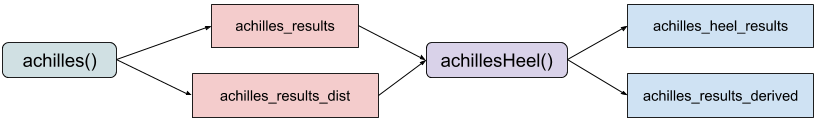
\includegraphics{../inst/doc/achilles_flowchart.png}

\subsection{SQL Only Mode}\label{sql-only-mode}

In most Achilles functions, you can specify \texttt{sqlOnly\ =\ TRUE} in
order to produce the SQL without executing it, which can be useful if
you'd like to examine the SQL closely or debug something. The SQL files
are stored in the \texttt{outputFolder}.

\subsection{Logging}\label{logging}

File and console logging is enabled across most Achilles functions. The
status of each step is logged into files in the \texttt{outputFolder}.
You can review the files in a common text editor, or use the Shiny
Application from the \texttt{ParallelLogger} package to view them more
interactively.

\begin{Shaded}
\begin{Highlighting}[]
\NormalTok{ParallelLogger}\OperatorTok{::}\KeywordTok{launchLogViewer}\NormalTok{(}\DataTypeTok{logFileName =} \StringTok{"output/log_achilles.txt"}\NormalTok{)}
\end{Highlighting}
\end{Shaded}

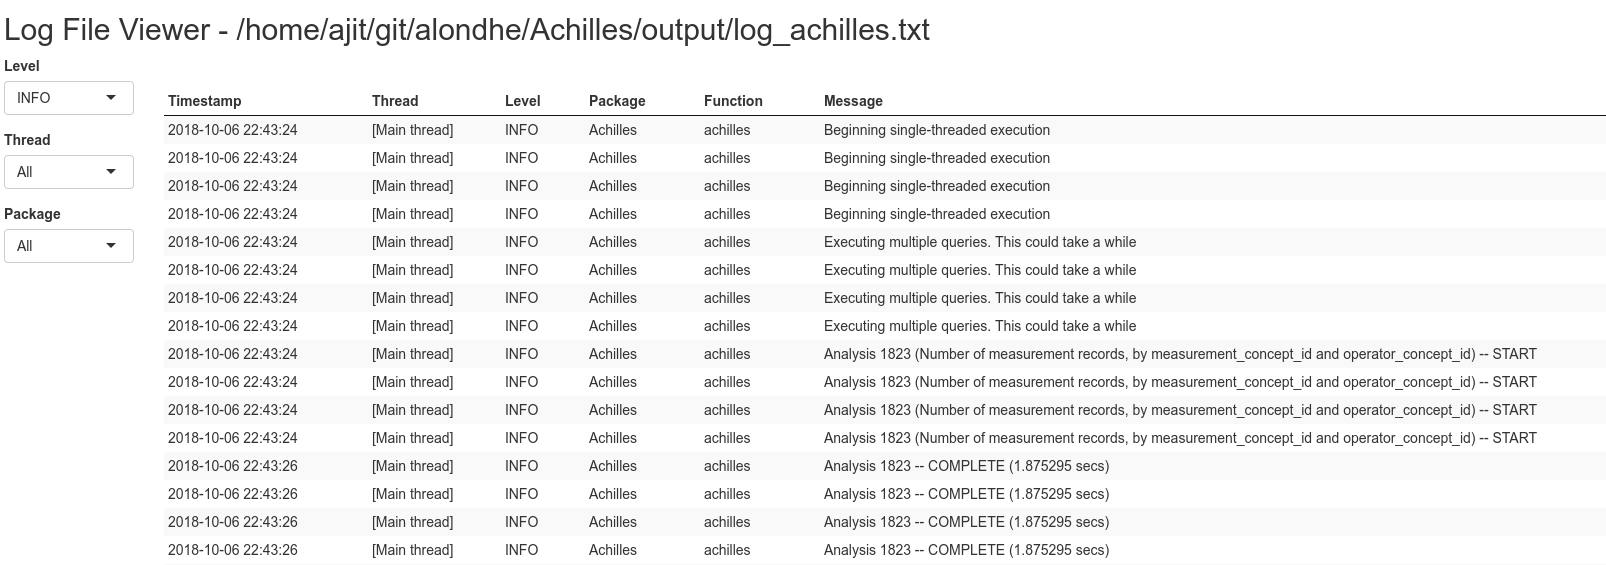
\includegraphics{../inst/doc/logging_screenshot.png}

\subsection{Verbose Mode}\label{verbose-mode}

The \texttt{verboseMode} parameter can be set to FALSE if you'd like
less details about the function execution to appear in the console.
Either way, all details are written to the log files. By default, this
is set to TRUE.

\subsection{Preparation for running
Achilles}\label{preparation-for-running-achilles}

In order to run the package, you will need to determine if you'd like
the Achilles tables and staging tables to be stored in schemas that are
separate from your CDM's schema (recommended), or within the same schema
as the CDM.

\subsubsection{Multi-Threaded vs
Single-Threaded}\label{multi-threaded-vs-single-threaded}

As the \textbf{achilles} and most of the \textbf{achillesHeel} functions
can run independently, we have added a multi-threaded mode to allow for
more than 1 SQL script to execute at a time. This is particularly useful
for massively parallel processing (MPP) platforms such as Amazon
Redshift and Microsoft PDW. It may not be beneficial for traditional SQL
platforms, so only use the multi-threaded mode if confident it can be
useful.

Further, while multiple threads can help performance in MPP platforms,
there can be diminishing returns as the cluster has a finite number of
concurrency slots to handle the queries. A rule of thumb: most likely
you should not use more than 10.

In the multi-threaded mode, all scripts produce permanent staging
tables, whereas in the single-threaded mode, the scripts produce
temporary staging tables. In both, the staging tables are merged to
produce the final Achilles tables.

\subsubsection{Validate your CDM schema}\label{validate-your-cdm-schema}

Before you run \textbf{achilles}, it may be useful to verify that your
CDM schema conforms to the OMOP CDM specification. This can quickly
identify issues with your CDM ahead of time. Refer to the
\href{https://github.com/OHDSI/CommonDataModel}{Common Data Model repo}
to identify which version of the CDM you intend to validate against.

\begin{Shaded}
\begin{Highlighting}[]
\NormalTok{connectionDetails <-}\StringTok{ }\KeywordTok{createConnectionDetails}\NormalTok{(}\DataTypeTok{dbms =} \StringTok{"postgresql"}\NormalTok{, }
                                             \DataTypeTok{server =} \StringTok{"localhost/synpuf"}\NormalTok{, }
                                             \DataTypeTok{user =} \StringTok{"cdm_user"}\NormalTok{, }
                                             \DataTypeTok{password =} \StringTok{"cdm_password"}\NormalTok{)}

\KeywordTok{validateSchema}\NormalTok{(}\DataTypeTok{connectionDetails =}\NormalTok{ connectionDetails, }
               \DataTypeTok{cdmDatabaseSchema =} \StringTok{"cdm"}\NormalTok{, }
               \DataTypeTok{resultsDatabaseSchema =} \StringTok{"results"}\NormalTok{, }
               \DataTypeTok{cdmVersion =} \FloatTok{5.3}\NormalTok{, }
               \DataTypeTok{runCostAnalysis =} \OtherTok{TRUE}\NormalTok{, }
               \DataTypeTok{outputFolder =} \StringTok{"output"}\NormalTok{, }
               \DataTypeTok{sqlOnly =} \OtherTok{FALSE}\NormalTok{)}
\end{Highlighting}
\end{Shaded}

\section{Achilles Parameters (Both
Modes)}\label{achilles-parameters-both-modes}

The following sub-sections describe the optional parameters in
\textbf{achilles} that can be configured, regardless of whether you run
the function in single- or multi-threaded mode.

\subsection{Staging Table Prefix}\label{staging-table-prefix}

To keep the staging tables organized, the \textbf{achilles} function
will use a table prefix of ``tmpach'' by default, but you can choose a
different one using the \texttt{tempAchillesPrefix} parameter. This is
useful for database platforms like Oracle, which limit the length of
table names.

\subsection{Source Name}\label{source-name}

The \texttt{sourceName} parameter is used to assign the name of the
dataset to the Achilles results. It is used in the Dashboard page in
AchillesWeb and Atlas Data Sources. If you set this to \texttt{NULL},
the \textbf{achilles} function will try to obtain the source name from
the CDM\_SOURCE table.

\subsection{Create Table}\label{create-table}

The \texttt{createTable} parameter, when set to \texttt{TRUE}, drops any
existing Achilles results tables and builds new ones. If set to
\texttt{FALSE}, these tables will persist, and the \textbf{achilles}
function will just insert new data to them.

\subsection{Limiting the Analyses}\label{limiting-the-analyses}

By default, the \textbf{achilles} function runs all analyses detailed in
the \texttt{getAnalysisDetails} function. However, it may be useful to
focus on a subset of analyses rather than running the whole set. This
can be accomplished by specifying analysis Ids in the
\texttt{analysisIds} parameter.

\subsection{Cost Analyses}\label{cost-analyses}

By default, the \textbf{achilles} function does not run analyses on the
COST table(s), as they can be very time-consuming, and are not critical
to most OHDSI studies. However, you can choose to run these analyses by
setting \texttt{runCostAnalysis} to \texttt{TRUE}. The cost analyses are
conditional on the CDM version. If using CDM v5.0, then the older cost
tables are queried. If using any version after 5.0, the unified cost
table is queried.

\subsection{Small Cell Count}\label{small-cell-count}

To avoid patient identifiability, you can establish the minimum cell
size that should be kept in the Achilles tables. Cells with small counts
(less than or equal to the value of the \texttt{smallCellCount}
parameter) are deleted. By default, this is set to 5. However, set to
NULL if you don't want any deletions.

\subsection{Drop Scratch Tables}\label{drop-scratch-tables}

\emph{See the Post-Processing section to read about how to run this step
separately}

\emph{This parameter is only necessary if running in multi-threaded
mode}

The \texttt{dropScratchTables} parameter, if set to \texttt{TRUE}, will
drop all staging tables created during the execution of
\textbf{achilles} in multi-threaded mode.

\subsection{Concept Hierarchy}\label{concept-hierarchy}

\emph{See the Post-Processing section to read about how to run this step
separately}

\emph{This table is only necessary if using Atlas Data Sources to
consume Achilles results}

The \texttt{conceptHierarchy} parameter, if set to \texttt{TRUE}, will
result in the concpet\_hierarchy table to be created in the results
schema.

\subsection{Create Indices}\label{create-indices}

\emph{See the Post-Processing section to read about how to run this step
separately}

The \texttt{createIndices} parameter, if set to \texttt{TRUE}, will
result in indices on the Achilles results tables to be created in order
to improve query performance.

\subsection{Return Value}\label{return-value}

When running \textbf{achilles}, the return value, if you assign a
variable to the function call, is a list object in which metadata about
the execution and all of the SQL scripts executed are attributes. You
can also run the function call without assigning a variable to it, so
that no values are printed or returned.

\section{Running Achilles: Single-Threaded
Mode}\label{running-achilles-single-threaded-mode}

In single-threaded mode, there is no need to set a
\texttt{scratchDatabaseSchema}, as temporary tables will be used.

\begin{Shaded}
\begin{Highlighting}[]
\NormalTok{connectionDetails <-}\StringTok{ }\KeywordTok{createConnectionDetails}\NormalTok{(}\DataTypeTok{dbms =} \StringTok{"postgresql"}\NormalTok{, }
                                             \DataTypeTok{server =} \StringTok{"localhost/synpuf"}\NormalTok{, }
                                             \DataTypeTok{user =} \StringTok{"cdm_user"}\NormalTok{, }
                                             \DataTypeTok{password =} \StringTok{"cdm_password"}\NormalTok{)}

\KeywordTok{achilles}\NormalTok{(}\DataTypeTok{connectionDetails =}\NormalTok{ connectionDetails, }
         \DataTypeTok{cdmDatabaseSchema =} \StringTok{"cdm"}\NormalTok{, }
         \DataTypeTok{resultsDatabaseSchema =} \StringTok{"results"}\NormalTok{, }
         \DataTypeTok{vocabDatabaseSchema =} \StringTok{"vocab"}\NormalTok{, }
         \DataTypeTok{sourceName =} \StringTok{"Synpuf"}\NormalTok{, }
         \DataTypeTok{cdmVersion =} \FloatTok{5.3}\NormalTok{, }
         \DataTypeTok{numThreads =} \DecValTok{1}\NormalTok{)}
\end{Highlighting}
\end{Shaded}

\section{Running Achilles: Multi-Threaded
Mode}\label{running-achilles-multi-threaded-mode}

In multi-threaded mode, you need to specify
\texttt{scratchDatabaseSchema} and use \textgreater{} 1 for
\texttt{numThreads}.

\begin{Shaded}
\begin{Highlighting}[]
\NormalTok{connectionDetails <-}\StringTok{ }\KeywordTok{createConnectionDetails}\NormalTok{(}\DataTypeTok{dbms =} \StringTok{"postgresql"}\NormalTok{, }
                                             \DataTypeTok{server =} \StringTok{"localhost/synpuf"}\NormalTok{, }
                                             \DataTypeTok{user =} \StringTok{"cdm_user"}\NormalTok{, }
                                             \DataTypeTok{password =} \StringTok{"cdm_password"}\NormalTok{)}

\KeywordTok{achilles}\NormalTok{(}\DataTypeTok{connectionDetails =}\NormalTok{ connectionDetails, }
         \DataTypeTok{cdmDatabaseSchema =} \StringTok{"cdm"}\NormalTok{, }
         \DataTypeTok{resultsDatabaseSchema =} \StringTok{"results"}\NormalTok{, }
         \DataTypeTok{scratchDatabaseSchema =} \StringTok{"scratch"}\NormalTok{, }
         \DataTypeTok{vocabDatabaseSchema =} \StringTok{"vocab"}\NormalTok{, }
         \DataTypeTok{sourceName =} \StringTok{"Synpuf"}\NormalTok{, }
         \DataTypeTok{cdmVersion =} \FloatTok{5.3}\NormalTok{, }
         \DataTypeTok{numThreads =} \DecValTok{5}\NormalTok{)}
\end{Highlighting}
\end{Shaded}

\section{Achilles Heel Parameters (Both
Modes)}\label{achilles-heel-parameters-both-modes}

\subsection{Staging Table Prefix}\label{staging-table-prefix-1}

To keep the staging tables organized, the \textbf{achillesHeel} function
will use a table prefix of ``tmpheel'' by default, but you can choose a
different one using the \texttt{tempHeelPrefix} parameter. This is
useful for database platforms like Oracle, which limit the length of
table names.

\subsection{Drop Scratch Tables}\label{drop-scratch-tables-1}

\emph{See the Post-Processing section to read about how to run this step
separately}

\emph{This parameter is only necessary if running in multi-threaded
mode}

The \texttt{dropScratchTables} parameter, if set to \texttt{TRUE} will
drop all staging tables created during the execution of
\textbf{achillesHeel} in multi-threaded mode.

\subsection{Thresholds}\label{thresholds}

The \texttt{ThresholdAgeWarning}, \texttt{ThresholdOutpatientVisitPerc},
and \texttt{ThresholdMinimalPtMeasDxRx} parameters can be used to
configure DQ thresholds in \textbf{achillesHeel}.

\begin{itemize}
\tightlist
\item
  \texttt{ThresholdAgeWarning} refers to the maximum age to allow in the
  dataset; by default, this is 125 years of age.
\item
  \texttt{ThresholdOutpatientVisitPerc} refers to the maximum percentage
  of outpatient visits allowed among all visits. This is by default set
  to 0.43.
\item
  \texttt{ThresholdMinimalPtMeasDxRx} refers to the minimum percentage
  required of patients with at least 1 measurement, 1 condition, and 1
  drug exposure. This is by default set to 20.5\%.
\end{itemize}

\section{Running Achilles Heel: Single-Threaded
Mode}\label{running-achilles-heel-single-threaded-mode}

In single-threaded mode, there is no need to set a
\texttt{scratchDatabaseSchema}, as temporary tables will be used.

\begin{Shaded}
\begin{Highlighting}[]
\NormalTok{connectionDetails <-}\StringTok{ }\KeywordTok{createConnectionDetails}\NormalTok{(}\DataTypeTok{dbms =} \StringTok{"postgresql"}\NormalTok{, }
                                             \DataTypeTok{server =} \StringTok{"localhost/synpuf"}\NormalTok{, }
                                             \DataTypeTok{user =} \StringTok{"cdm_user"}\NormalTok{, }
                                             \DataTypeTok{password =} \StringTok{"cdm_password"}\NormalTok{)}

\KeywordTok{achillesHeel}\NormalTok{(}\DataTypeTok{connectionDetails =}\NormalTok{ connectionDetails, }
             \DataTypeTok{cdmDatabaseSchema =} \StringTok{"cdm"}\NormalTok{, }
             \DataTypeTok{resultsDatabaseSchema =} \StringTok{"results"}\NormalTok{, }
             \DataTypeTok{vocabDatabaseSchema =} \StringTok{"vocab"}\NormalTok{, }
             \DataTypeTok{cdmVersion =} \FloatTok{5.3}\NormalTok{, }
             \DataTypeTok{numThreads =} \DecValTok{1}\NormalTok{, }
             \DataTypeTok{outputFolder =} \StringTok{"output"}\NormalTok{)}
\end{Highlighting}
\end{Shaded}

\section{Running Achilles Heel: Multi-Threaded
Mode}\label{running-achilles-heel-multi-threaded-mode}

In multi-threaded mode, you need to specify
\texttt{scratchDatabaseSchema} and use \textgreater{} 1 for
\texttt{numThreads}.

\begin{Shaded}
\begin{Highlighting}[]
\NormalTok{connectionDetails <-}\StringTok{ }\KeywordTok{createConnectionDetails}\NormalTok{(}\DataTypeTok{dbms =} \StringTok{"postgresql"}\NormalTok{, }
                                             \DataTypeTok{server =} \StringTok{"localhost/synpuf"}\NormalTok{, }
                                             \DataTypeTok{user =} \StringTok{"cdm_user"}\NormalTok{, }
                                             \DataTypeTok{password =} \StringTok{"cdm_password"}\NormalTok{)}
\KeywordTok{achillesHeel}\NormalTok{(}\DataTypeTok{connectionDetails =}\NormalTok{ connectionDetails, }
             \DataTypeTok{cdmDatabaseSchema =} \StringTok{"cdm"}\NormalTok{, }
             \DataTypeTok{resultsDatabaseSchema =} \StringTok{"results"}\NormalTok{, }
             \DataTypeTok{vocabDatabaseSchema =} \StringTok{"vocab"}\NormalTok{, }
             \DataTypeTok{cdmVersion =} \FloatTok{5.3}\NormalTok{, }
             \DataTypeTok{numThreads =} \DecValTok{5}\NormalTok{, }
             \DataTypeTok{outputFolder =} \StringTok{"output"}\NormalTok{, }
             \DataTypeTok{scratchDatabaseSchema =} \StringTok{"scratch"}\NormalTok{)}
\end{Highlighting}
\end{Shaded}

\section{Post-Processing}\label{post-processing}

This section describes the usage of standalone functions for
post-processing that can be invoked if you did not use them in the
\textbf{achilles} function call.

\subsection{Creating the Concept Hierarchy: Single-Threaded
Mode}\label{creating-the-concept-hierarchy-single-threaded-mode}

\emph{This table is only necessary if using Atlas Data Sources to
consume Achilles results}

In single-threaded mode, there is no need to set a
\texttt{scratchDatabaseSchema}, as temporary tables will be used.

\begin{Shaded}
\begin{Highlighting}[]
\NormalTok{connectionDetails <-}\StringTok{ }\KeywordTok{createConnectionDetails}\NormalTok{(}\DataTypeTok{dbms =} \StringTok{"postgresql"}\NormalTok{, }
                                             \DataTypeTok{server =} \StringTok{"localhost/synpuf"}\NormalTok{, }
                                             \DataTypeTok{user =} \StringTok{"cdm_user"}\NormalTok{, }
                                             \DataTypeTok{password =} \StringTok{"cdm_password"}\NormalTok{)}

\KeywordTok{createConceptHierarchy}\NormalTok{(}\DataTypeTok{connectionDetails =}\NormalTok{ connectionDetails, }
                       \DataTypeTok{resultsDatabaseSchema =} \StringTok{"results"}\NormalTok{, }
                       \DataTypeTok{vocabDatabaseSchema =} \StringTok{"vocab"}\NormalTok{, }
                       \DataTypeTok{outputFolder =} \StringTok{"output"}\NormalTok{)}
\end{Highlighting}
\end{Shaded}

\subsection{Creating the Concept Hierarchy: Multi-Threaded
Mode}\label{creating-the-concept-hierarchy-multi-threaded-mode}

\emph{This table is only necessary if using Atlas Data Sources to
consume Achilles results}

In multi-threaded mode, you need to specify
\texttt{scratchDatabaseSchema} and use \textgreater{} 1 for
\texttt{numThreads}.

\begin{Shaded}
\begin{Highlighting}[]
\NormalTok{connectionDetails <-}\StringTok{ }\KeywordTok{createConnectionDetails}\NormalTok{(}\DataTypeTok{dbms =} \StringTok{"postgresql"}\NormalTok{, }
                                             \DataTypeTok{server =} \StringTok{"localhost/synpuf"}\NormalTok{, }
                                             \DataTypeTok{user =} \StringTok{"cdm_user"}\NormalTok{, }
                                             \DataTypeTok{password =} \StringTok{"cdm_password"}\NormalTok{)}

\KeywordTok{createConceptHierarchy}\NormalTok{(}\DataTypeTok{connectionDetails =}\NormalTok{ connectionDetails, }
                       \DataTypeTok{resultsDatabaseSchema =} \StringTok{"results"}\NormalTok{, }
                       \DataTypeTok{vocabDatabaseSchema =} \StringTok{"vocab"}\NormalTok{, }
                       \DataTypeTok{outputFolder =} \StringTok{"output"}\NormalTok{, }
                       \DataTypeTok{scratchDatabaseSchema =} \StringTok{"scratch"}\NormalTok{, }
                       \DataTypeTok{numThreads =} \DecValTok{3}\NormalTok{)}
\end{Highlighting}
\end{Shaded}

\subsection{Creating Indices}\label{creating-indices}

\emph{Not supported by Amazon Redshift or IBM Netezza; function will
skip this step if using those platforms}

To improve query performance of the Achilles results tables, run the
\textbf{createIndices} function.

\begin{Shaded}
\begin{Highlighting}[]
\NormalTok{connectionDetails <-}\StringTok{ }\KeywordTok{createConnectionDetails}\NormalTok{(}\DataTypeTok{dbms =} \StringTok{"postgresql"}\NormalTok{, }
                                             \DataTypeTok{server =} \StringTok{"localhost/synpuf"}\NormalTok{, }
                                             \DataTypeTok{user =} \StringTok{"cdm_user"}\NormalTok{, }
                                             \DataTypeTok{password =} \StringTok{"cdm_password"}\NormalTok{)}

\KeywordTok{createIndices}\NormalTok{(}\DataTypeTok{connectionDetails =}\NormalTok{ connectionDetails, }
              \DataTypeTok{resultsDatabaseSchema =} \StringTok{"results"}\NormalTok{, }
              \DataTypeTok{outputFolder =} \StringTok{"output"}\NormalTok{)}
\end{Highlighting}
\end{Shaded}

\subsection{Dropping All Staging Tables (Multi-threaded
only)}\label{dropping-all-staging-tables-multi-threaded-only}

If the \textbf{achilles} or \textbf{achillesHeel} execution has errors,
or if you did not enable this step in the call to these functions, use
the \texttt{dropAllScratchTables} function.

The \texttt{tableTypes} parameter can be used to specify which batch of
staging tables to drop (``achilles'', ``heel'', ``concept\_hierarchy'').
The default value is to drop them all.

\begin{Shaded}
\begin{Highlighting}[]
\NormalTok{connectionDetails <-}\StringTok{ }\KeywordTok{createConnectionDetails}\NormalTok{(}\DataTypeTok{dbms =} \StringTok{"postgresql"}\NormalTok{, }
                                             \DataTypeTok{server =} \StringTok{"localhost/synpuf"}\NormalTok{, }
                                             \DataTypeTok{user =} \StringTok{"cdm_user"}\NormalTok{, }
                                             \DataTypeTok{password =} \StringTok{"cdm_password"}\NormalTok{)}

\KeywordTok{dropAllScratchTables}\NormalTok{(}\DataTypeTok{connectionDetails =}\NormalTok{ connectionDetails, }
                     \DataTypeTok{scratchDatabaseSchema =} \StringTok{"scratch"}\NormalTok{, }\DataTypeTok{numThreads =} \DecValTok{5}\NormalTok{)}
\end{Highlighting}
\end{Shaded}

\section{Examining the Heel Results}\label{examining-the-heel-results}

To view the Heel results, you can use the fetchAchillesHeelResults()
function or the launchHeelResultsViewer() function. The former produces
an R data frame that you can then export to various formats. The latter
launches a Shiny application that renders the results in an easy to
consume HTML file that can be viewed in your internet browser.

Heel Results are warnings split into 3 categories:

\begin{itemize}
\tightlist
\item
  \textbf{ERROR}: Something is probably not right with the way you
  transformed your native dataset into the CDM dataset. Review the error
  message and the associated Achilles analysis Id and Heel rule Id to
  investigate further. Use the \textbf{getAnalysisDetails} function to
  identify the Achilles analysis, and use the
  \textbf{fetchAchillesAnalysisResults} function to view the exact
  results of that analysis. Additionally, the
  \textbf{launchHeelResultsViewer} function launches a Shiny Application
  that can directly provide you with the associated SQL scripts.
\item
  \textbf{WARNING}: Something \emph{may} be an issue with the domain or
  concept associated with the Achilles analysis Id or Heel rule Id.
  However, not all datasets are the same; Achilles Heel tries to compare
  yours to a gold-standard dataset, so it is very likely you will
  encounter some WARNINGs. Feel free to ignore these WARNINGs if they
  are acceptable deviations from the gold-standard, but it is good
  practice to document these deviations for other researchers'
  knowledge.
\item
  \textbf{NOTIFICATION}: These messages simply tell you how your
  dataset's content compares to practical thresholds on things like age,
  concept counts, death events, and visit types. These thresholds are
  not necessarily gold-standard, just values that are thought to be
  reasonable expected minimums or maximums. Feel free to ignore these
  NOTIFICATIONs if the expected values do not make sense with your
  particular dataset.
\end{itemize}

\subsection{Fetch a data frame with the Heel
Results}\label{fetch-a-data-frame-with-the-heel-results}

Once \textbf{achillesHeel} is run, you can fetch the results into a data
frame for further consumption into whichever format you like using the
\textbf{fetchAchillesHeelResults} function.

\begin{Shaded}
\begin{Highlighting}[]
\NormalTok{connectionDetails <-}\StringTok{ }\KeywordTok{createConnectionDetails}\NormalTok{(}\DataTypeTok{dbms =} \StringTok{"postgresql"}\NormalTok{, }
                                             \DataTypeTok{server =} \StringTok{"localhost/synpuf"}\NormalTok{, }
                                             \DataTypeTok{user =} \StringTok{"cdm_user"}\NormalTok{, }
                                             \DataTypeTok{password =} \StringTok{"cdm_password"}\NormalTok{)}

\KeywordTok{fetchAchillesHeelResults}\NormalTok{(}\DataTypeTok{connectionDetails =}\NormalTok{ connectionDetails, }
                         \DataTypeTok{resultsDatabaseSchema =} \StringTok{"results"}\NormalTok{)}
\end{Highlighting}
\end{Shaded}

\subsection{View Heel Results in Interactive Shiny
Application}\label{view-heel-results-in-interactive-shiny-application}

The Heel Results Shiny Application can be useful in interacting with the
Heel Results. The Heel warnings are color-coded based on severity
(``ERROR'', ``WARNING'', ``NOTIFICATION''), and are searchable. You can
also click on a row to see the associated Analysis and Heel SQL scripts
to try to debug the root cause. Results can be downloaded to CSV using
the ``Download Heel Results'' button.

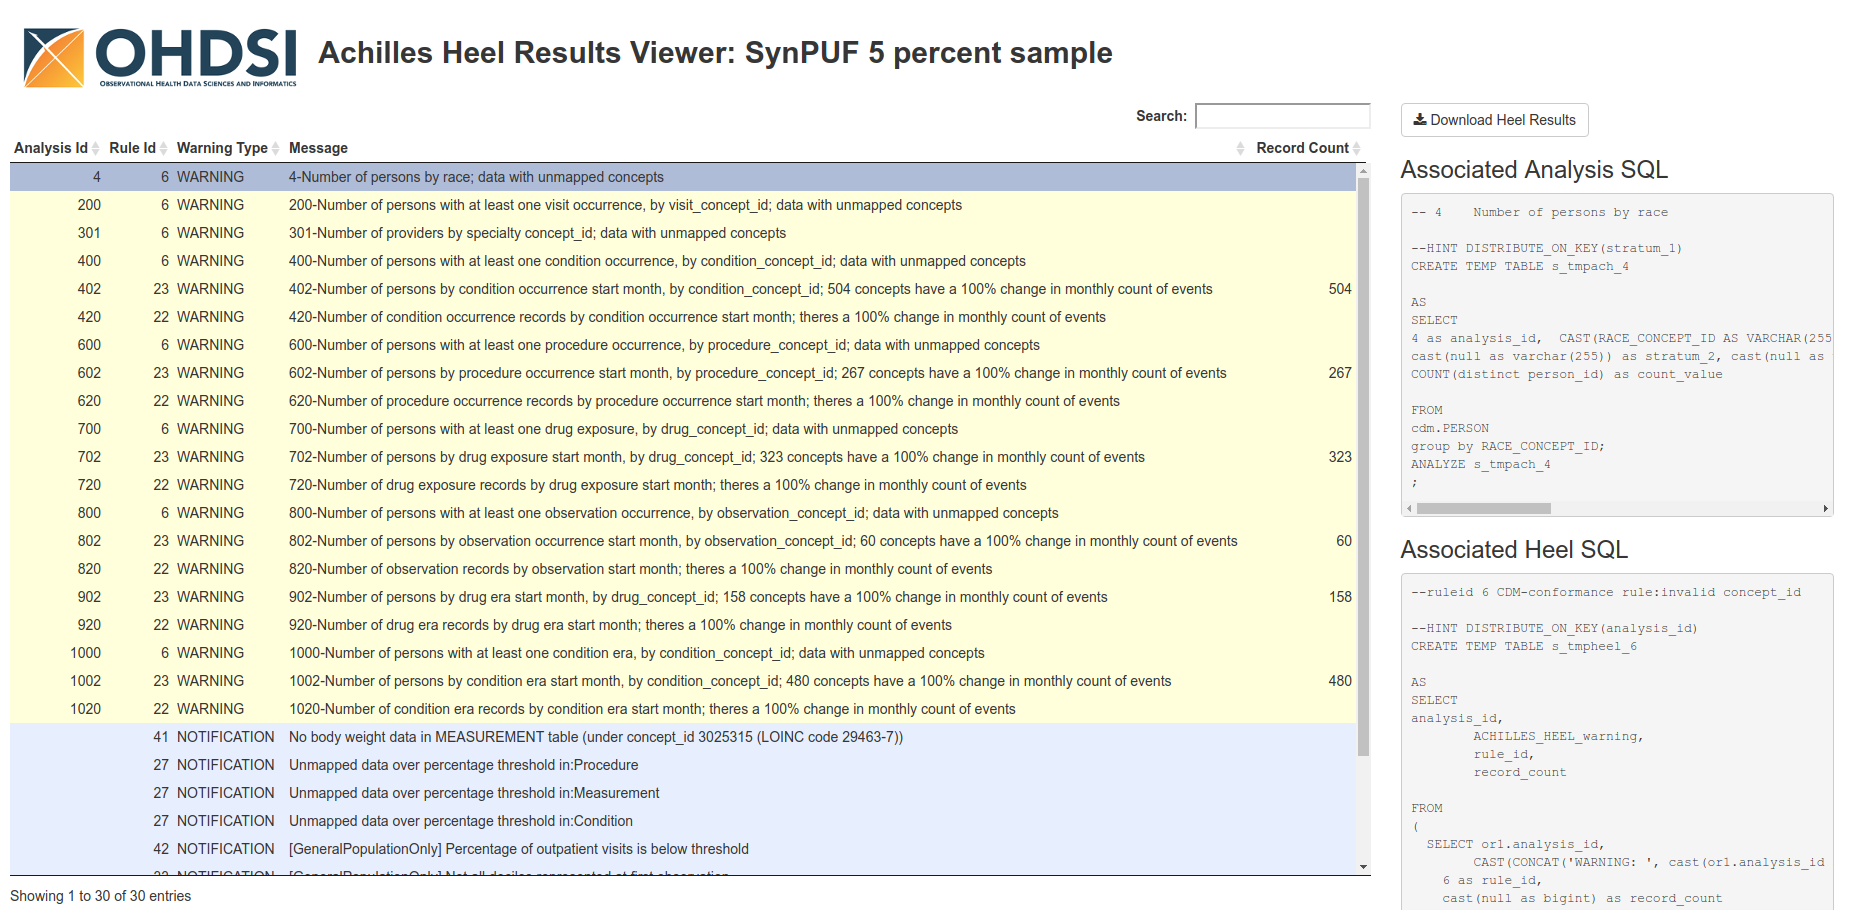
\includegraphics{../inst/doc/shinyHeel_screenshot.png}

When calling \textbf{launchHeelResultsViewer}, use the same parameters
you used to execute \textbf{achilles} and \textbf{achillesHeel}. The
Shiny app will use the parameters to render and translate the associated
SQL scripts so that you can copy and run them separately to debug
issues.

\begin{Shaded}
\begin{Highlighting}[]
\NormalTok{connectionDetails <-}\StringTok{ }\NormalTok{DatabaseConnector}\OperatorTok{::}\KeywordTok{createConnectionDetails}\NormalTok{(}\DataTypeTok{dbms =} \StringTok{"postgresql"}\NormalTok{, }
                                                                \DataTypeTok{server =} \StringTok{"localhost/synpuf"}\NormalTok{, }
                                                                \DataTypeTok{user =} \StringTok{"cdm_user"}\NormalTok{, }
                                                                \DataTypeTok{password =} \StringTok{"cdm_password"}\NormalTok{)}
\KeywordTok{launchHeelResultsViewer}\NormalTok{(}\DataTypeTok{connectionDetails =}\NormalTok{ connectionDetails, }
                        \DataTypeTok{cdmDatabaseSchema =} \StringTok{"cdm"}\NormalTok{, }
                        \DataTypeTok{resultsDatabaseSchema =} \StringTok{"results"}\NormalTok{, }
                        \DataTypeTok{scratchDatabaseSchema =} \StringTok{"scratch"}\NormalTok{,}
                        \DataTypeTok{outputFolder =} \StringTok{"output"}\NormalTok{, }
                        \DataTypeTok{numThreads =} \DecValTok{5}\NormalTok{)}
\end{Highlighting}
\end{Shaded}

\subsection{Using AchillesWeb}\label{using-achillesweb}

AchillesWeb is a lightweight web application that can be used to consume
the Achilles and Heel results graphically. It is no longer actively
updated, as development priorities have shifted towards Atlas Data
Sources, but AchillesWeb can still be utilized. To connect Achilles
results to AchillesWeb, the Achilles results need to be exported to JSON
files and the AchillesWeb JSON file needs to point to those JSON files.

Please refer to \href{https://github.com/OHDSI/AchillesWeb}{AchillesWeb}
for more information.

\subsubsection{Exporting to JSON}\label{exporting-to-json}

The \texttt{exportToJson} function can export all of the Achilles
results to JSON files that AchillesWeb can consume.

\begin{itemize}
\tightlist
\item
  The \texttt{compressIntoOnFile} parameter, if set to \texttt{TRUE},
  will compress all of the files into one zip file for easier
  portability.
\item
  The \texttt{reports} parameter can be used to export specific reports
  rather than all. Use the \texttt{showReportTypes} function to see all
  possible reports.
\end{itemize}

\begin{Shaded}
\begin{Highlighting}[]
\NormalTok{connectionDetails <-}\StringTok{ }\KeywordTok{createConnectionDetails}\NormalTok{(}\DataTypeTok{dbms =} \StringTok{"postgresql"}\NormalTok{, }
                                             \DataTypeTok{server =} \StringTok{"localhost/synpuf"}\NormalTok{, }
                                             \DataTypeTok{user =} \StringTok{"cdm_user"}\NormalTok{, }
                                             \DataTypeTok{password =} \StringTok{"cdm_password"}\NormalTok{)}

\KeywordTok{exportToJson}\NormalTok{(}\DataTypeTok{connectionDetails =}\NormalTok{ connectionDetails, }
             \DataTypeTok{cdmDatabaseSchema =} \StringTok{"cdm"}\NormalTok{, }
             \DataTypeTok{resultsDatabaseSchema =} \StringTok{"results"}\NormalTok{, }
             \DataTypeTok{outputPath =} \StringTok{"output"}\NormalTok{, }
             \DataTypeTok{vocabDatabaseSchema =} \StringTok{"vocab"}\NormalTok{)}
\end{Highlighting}
\end{Shaded}

\subsubsection{Adding Data Sources to
AchillesWeb}\label{adding-data-sources-to-achillesweb}

AchillesWeb relies upon a JSON file to point to CDM Achilles result JSON
files.

\begin{Shaded}
\begin{Highlighting}[]
\KeywordTok{addDataSource}\NormalTok{(}\DataTypeTok{jsonFolderPath =} \StringTok{"output"}\NormalTok{, }
              \DataTypeTok{dataSourcePath =} \StringTok{"achillesWeb"}\NormalTok{)}
\end{Highlighting}
\end{Shaded}

\subsection{Using Atlas Data Sources}\label{using-atlas-data-sources}

If the Achilles results tables and the concept\_hierarchy table are
present in the results schema, you can point Atlas to this schema to
have the results appear graphically in Atlas Data Sources.

Please refer to \href{https://github.com/OHDSI/Atlas}{Atlas Data
Sources} for more information.

\section{Acknowledgments}\label{acknowledgments}

Considerable work has been dedicated to provide the \texttt{Achilles}
package.

\begin{Shaded}
\begin{Highlighting}[]
\KeywordTok{citation}\NormalTok{(}\StringTok{"Achilles"}\NormalTok{)}
\end{Highlighting}
\end{Shaded}

\begin{verbatim}
#> 
#> To cite package 'Achilles' in publications use:
#> 
#>   Patrick Ryan, Martijn Schuemie, Vojtech Huser, Chris Knoll, Ajit
#>   Londhe and Taha Abdul-Basser (2018). Achilles: Creates
#>   Descriptive Statistics Summary for an Entire OMOP CDM Instance.
#>   R package version 1.6.3.
#> 
#> A BibTeX entry for LaTeX users is
#> 
#>   @Manual{,
#>     title = {Achilles: Creates Descriptive Statistics Summary for an Entire OMOP CDM Instance},
#>     author = {Patrick Ryan and Martijn Schuemie and Vojtech Huser and Chris Knoll and Ajit Londhe and Taha Abdul-Basser},
#>     year = {2018},
#>     note = {R package version 1.6.3},
#>   }
\end{verbatim}


\end{document}
